\section{PostgreSQL}
PostgreSQL is an ORDBMS - abbreviation for open source object-relational database management system. Origins date back to the year 1986, where the project then known as POSTGRES started as a reference to the older INGRES database. One decade later it got renamed to PostgreSQL to clearly show its ability to work with SQL.\cite{PostgreSQL} 

Nowadays, it's widely used. PostgreSQL popularity has been steadily rising in the last few years. Based on "Stack Overflow Annual Developer Survey"~\cite{Stackoverflow survey}, PostgreSQL currently sits in second place for the 'Most popular technology in the database category', right after the MySQL.

\subsection{Parse tree}
PostgreSQL internally uses parse trees to process SQL Queries. The whole parsing comprises multiple stages. First, a query passed in form of plain text is transformed to tokens using a tool \textit{Flex}. Next up the parser generator called \textit{Flex} is used. It consists of multiple grammar rules and actions. Each action is executed whenever any of the rules are applied and together they are used to build the final parse tree.

\newpage

\begin{figure}[h]
  \makebox[\textwidth]{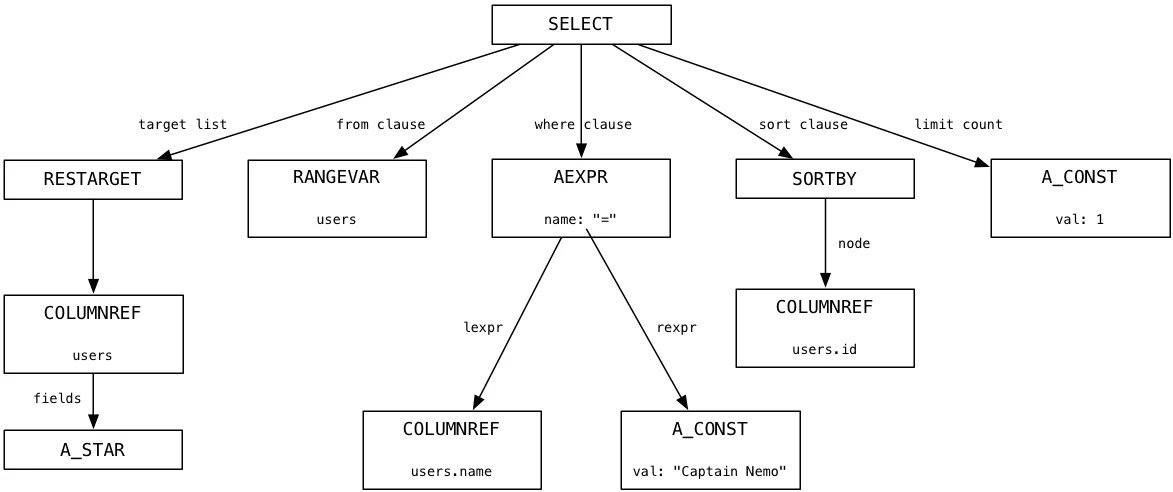
\includegraphics[width=\textwidth]{parse_tree.jpg}}
  \caption {Visualisation of parse tree for \texttt{"SELECT * FROM users WHERE name = 'Captain Nemo' ORDER BY id ASC LIMIT 1"}}
\end{figure}

During the \textit{Parse stage}, the parser checks the syntax of a query string. It does not do any lookups in the system catalogs, and for that reason, it is independent of the database schema. In the following chapters you will see how our library seamlessly exposes the internal Postgres parse trees to the higher level language and how this can be used to validate queries during compilation.

\subsection{Reasons to use parse trees}
Having the option to work with parse tree directly, can prove useful in multiple cases. \cite{Parse tree usage}
\begin{description}[font=$\bullet$~\normalfont\scshape\color{black}\\]
\item [Extracting specific part of query] \hfill \newline
Using parse tree, we will be able to easily extract parts like column names from the \texttt{SELECT} target list, expression from the \texttt{WHERE} statement or nested statement from some complicated SQL query.
\item [Modifying part of the query string] \hfill \newline
In a similar fashion to extracting, we can also replace parts in the query. We can for example change the \texttt{sort\_clause} in \texttt{SELECT} statement or change the target columns of the query.
\item [Determining type of query] \hfill \newline
It can be also used to accomplish load balancing in applications, by deciding whether the query is read only, or it writes something into the database.
\end{description}